\begin{frame}{Week 2: Finite-State Acceptors}
\protect\hypertarget{week-2-finite-state-acceptors}{}
Textbook: 1.1 and 1.2
\end{frame}

\begin{frame}{Definitions}
\protect\hypertarget{definitions}{}
\begin{itemize}
\item
  An \textbf{automaton} (plural automata) is a self-moving machine. In
  this context, it just means ``small, simple, simulated machine''.
\item
  An \textbf{acceptor} is an automaton which takes in a string and
  either accepts or rejects it through a series of state transitions.
  \textbf{Note:} Many texts fail to distinguish between \emph{automata}
  and \emph{acceptors}. Acceptors are a proper subset of automata.
\item
  A \textbf{finite-state} automaton has a finite number of states that
  it can transition through. Infinite-state automata are not used.
\item
  A \textbf{deterministic} automaton has exactly one set of state
  transitions which follow from a given string. A nondeterministic one,
  on the other hand, has multiple series of state transitions which may
  follow.
\end{itemize}
\end{frame}

\begin{frame}{Kleene operators}
\protect\hypertarget{kleene-operators}{}
\begin{itemize}
\item
  For an alphabet \(\Sigma\), the \textbf{Kleene star} is an operator
  creating the set of all strings of zero or more characters
\item
  If \(\Sigma^i\) is the set of all strings of length \(i\) over
  \(\Sigma\), then \(\Sigma^* = \bigcup_{i = 0}^\infty \Sigma^i\)
\item
  Ex: \[
    \{ 0, 1 \}^* = \{ \epsilon, 0, 1, 00, 01, 10, 11, \ldots \}
    \]
\item
  The \textbf{Kleene plus} gives the set of all strings of \emph{one} or
  more characters over an alphabet. It is less common
\end{itemize}

\[
\Sigma^* = \Sigma^+ \cup \{ \epsilon \}
\]
\end{frame}

\begin{frame}{DFAs}
\protect\hypertarget{dfas}{}
\begin{itemize}
\tightlist
\item
  A \textbf{deterministic finite-state acceptor (DFA)} is an automaton
  built to accept strings using a finite number of states where each
  string corresponds to exactly one series of state transitions.
  Formally:
\end{itemize}

\textbf{Def:} Finite-state acceptor. A finite acceptor is a 5-tuple
\(A = (Q, \Sigma, \delta, q_0, F)\) where:

\begin{enumerate}
[1)]
\tightlist
\item
  Q is a finite set called the \textbf{states}
\item
  \(\Sigma\) is a finite set of symbols called the \textbf{alphabet}
\item
  \(\delta : ( Q \times \Sigma ) \to Q\) is the \textbf{transition
  function}
\item
  \(q_0 \in Q\) is the \textbf{start state}
\item
  \(F \subseteq Q\) is the set of acceptance states
\end{enumerate}

\textbf{Note:} A DFA must define all transitions! Every state must have
a specified target state for every character in the alphabet.
\end{frame}

\begin{frame}{DFA operation}
\protect\hypertarget{dfa-operation}{}
Consider the DFA \(A\) with states \(Q = \{ q_0, q_1, q_2 \}\), starting
state \(q_0\), alphabet \(\Sigma = \{ a, b, c \}\), and acceptance state
set \(F = \{ q_2 \}\). The following graph demonstrates \(\delta\).

\textbf{Note:} An arrow from nothing means ``initial state''. In these
diagrams, shading means ``accepting state''.

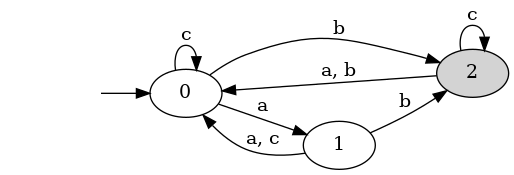
\includegraphics{figures/dfa_ex.png}

This will accept any string of the forms \(abc^i\) or \(bc^i\), where
\(i\) is any nonnegative integer.
\end{frame}

\begin{frame}{NFAs}
\protect\hypertarget{nfas}{}
\begin{itemize}
\tightlist
\item
  A \textbf{nondeterministic finite-state acceptor (NFA)} is a DFA that
  can follow multiple series of state transitions
\item
  The NFA accepts iff any of its branches do
\item
  The only formal difference is in the transition function:
  \textbf{\(\delta\) can output any number of output states}
\end{itemize}

\textbf{Def:} Nondeterministic finite-state acceptor (NFA). An NFA is a
5-tuple \(A = (Q, \Sigma, \delta, q_0, F)\) where:

\begin{enumerate}
[1)]
\tightlist
\item
  Q is a finite set called the states
\item
  \(\Sigma\) is a finite set of symbols called the alphabet
\item
  \(\delta : (Q \times \{ \Sigma \cup \epsilon \}) \to \mathcal{P}(Q)\)
  is the \textbf{nondeterministic transition function}
\item
  \(q_0 \in Q\) is the start state
\item
  \(F \subseteq Q\) is the set of acceptance states
\end{enumerate}

\textbf{Note:} If an NFA can leave transitions undefined, unlike a DFA.
If it comes to a fork in the road, it duplicates and goes down both
paths.
\end{frame}

\begin{frame}{NFA operation}
\protect\hypertarget{nfa-operation}{}
This NFA accepts the same language as our previous DFA:

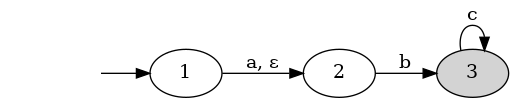
\includegraphics{figures/nfa_ex.png}

This NFA has more ``weird'' branches:

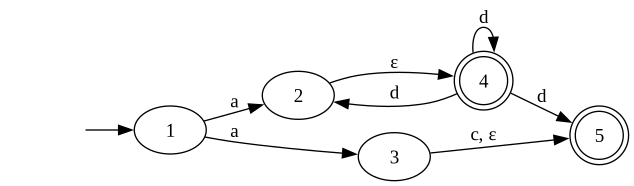
\includegraphics{figures/nfa_ex_2.png}
\end{frame}

\begin{frame}[fragile]{Practice problems}
\protect\hypertarget{practice-problems}{}
Do these problems on your own, then we will do them on the board.

\begin{enumerate}
[1)]
\tightlist
\item
  Does the following DFA accept \texttt{fizz}? \texttt{foo}?
  \texttt{buzz}?
\end{enumerate}

\includegraphics{figures/week1_p1.png}

\begin{enumerate}
[1)]
\setcounter{enumi}{1}
\tightlist
\item
  Describe the set of all strings accepted by the this NFA.
\end{enumerate}

\includegraphics{figures/week1_p2.png}

\begin{enumerate}
[1)]
\setcounter{enumi}{2}
\tightlist
\item
  Construct an NFA to recognize the set of all strings consisting of
  repetitions of \texttt{abc}.
\end{enumerate}
\end{frame}

\begin{frame}{DFA-NFA equivalence proof}
\protect\hypertarget{dfa-nfa-equivalence-proof}{}
\begin{itemize}
\tightlist
\item
  Counterintuitively, \textbf{NFA and DFA are equivalent}: Every DFA has
  an equivalent NFA and vice versa. We will prove this in two parts
  below.
\end{itemize}

\textbf{Thm:} All DFA have equivalent NFA. \textbf{Pf:} The set of all
DFA is a subset of the set of all NFA. Therefore, all DFA are trivially
NFA. End of proof.

\textbf{Thm:} All NFA have equivalent DFA. \textbf{Pf:} By construction.
DFA have \(\delta_\texttt{DFA}: (Q \times \Sigma) \to Q\), while NFA
have
\(\delta_\texttt{NFA}: (Q \times \{ \Sigma \cup \epsilon \}) \to \mathcal{P}(Q)\).
We will show that all \(\delta_\texttt{NFA}\) have an equivalent
modification in the form of \(\delta_\texttt{DFA}\), proving that all
NFA are equivalent to DFA.

\begin{enumerate}
[1)]
\item
  \(Q\) vs \(\mathcal{P}(Q)\). Since \(Q\) is a finite set,
  \(\mathcal{P}(Q)\) is a finite set of size \(2^{|Q|}\). Any finite set
  can be used as a set of DFA states, so \(\mathcal{P}(Q)\) works.
  \textbf{Let} \(Q^\prime = \mathcal{P}(Q)\).
\item
  \(\epsilon\) transitions. We must eliminate any nonconsumptive
  transitions in order to be a valid DFA. Let
  \(E: Q \to \mathcal{P}(Q)\) be the \textbf{\(\epsilon\)-closure}
  function mapping a state to the set all all states reachable by
  \(\epsilon\) transitions from it. Note that \(E: Q \to Q^\prime\).
  \textbf{Let}
  \(\delta^\prime(q, \sigma) = E(\delta_\texttt{NFA}(E(q), \sigma))\).
  Note that \(\delta^\prime : (Q^\prime \times \Sigma) \to Q^\prime\).
\item
  Starting states. The starting state may have outgoing \(\epsilon\)
  transitions which must be accounted for. Thus, \textbf{let}
  \(q_0^\prime = E(q_0)\).
\item
  Accepting states. An NFA's \(F\) is a subset of the set of its states
  (\(F \subset Q\)). However, it is not a subset of \(Q^\prime\) yet:
  Thus, we must adjust it. \textbf{Let}
  \(F^\prime = \{ R \in Q^\prime : R \texttt{ contains an accept state from } F \}\).
\end{enumerate}

Now, for an arbitrary NFA \(A = (Q, \Sigma, \delta, q_0, F)\), let
\(A^\prime = (Q^\prime, \Sigma, \delta^\prime, q_0^\prime, F^\prime)\).
By the above rules, \(A^\prime\) is a valid DFA equivalent to \(A\). End
of proof.
\end{frame}

\begin{frame}{The regular operations}
\protect\hypertarget{the-regular-operations}{}
\end{frame}

\begin{frame}{Next up: Regular languages}
\protect\hypertarget{next-up-regular-languages}{}
\end{frame}
